\section*{سوال ۴}

در یک فروشگاه تحت وب، کسب و کار مربوطه وظیفه واسطه‌گری را بر عهده دارد و تعداد زیادی مشتری را به تعداد زیادی انباردار متصل می‌کند. هم مشتریان و هم انبارداران در این سیستم دارای حساب و کیف پول هستند، و هر خرید به طور مستقیم پول را از کیف پول مشتری به کیف پول فروشنده منتقل می‌کند (بدون هیچ هزینه‌ای).

مدل زیرساختی که برای این فروشگاه تعریف شده است به عنوان مدل backend شناخته می‌شود و برای بخشی از کد زیرسیستم طراحی شده است. برای سهولت در توضیح سوال، بسیاری از جزئیات (داده‌ها و عملیات کلاس‌ها) حذف شده‌اند و تمرکز بر روی کلاس‌ها و روابط بین آن‌ها است.

\begin{figure}[h]
	\centering
	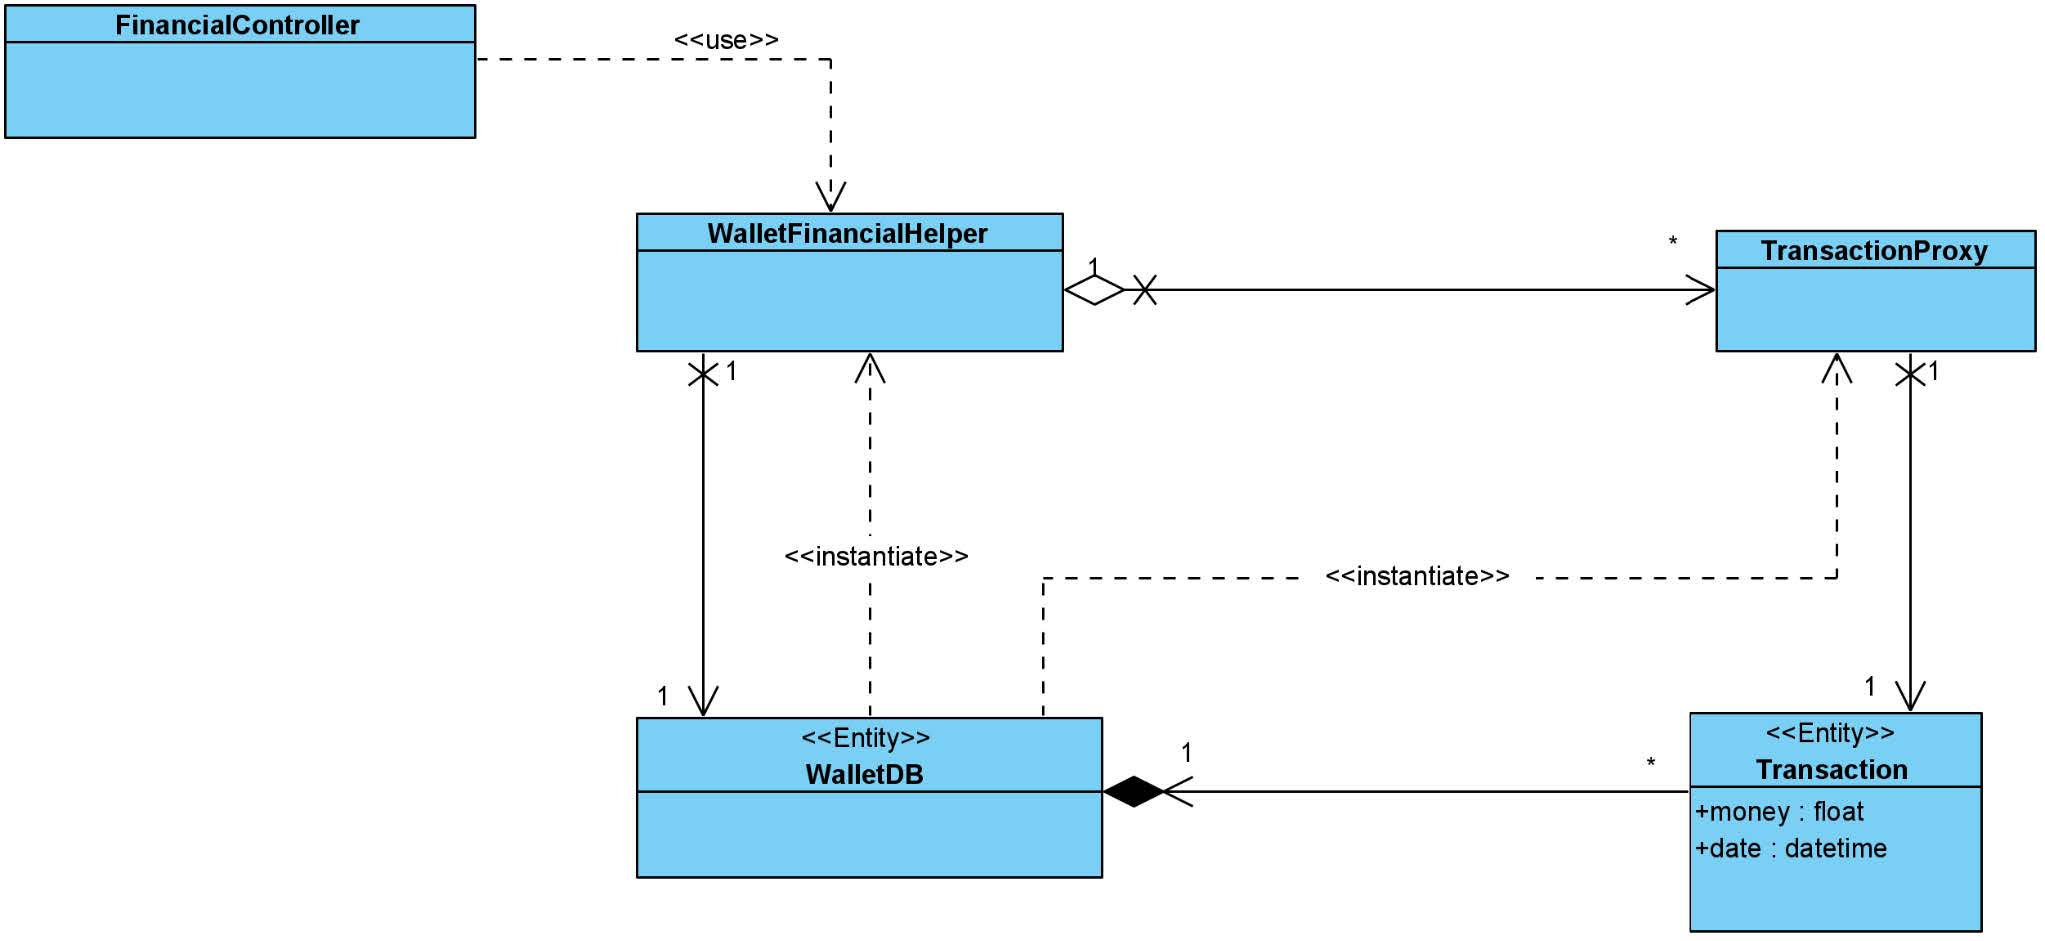
\includegraphics{pic1.jpg}
	\label{fig:label4}
\end{figure}

\subsection*{۱. بازسازی مدل تحلیل}
مدل تحلیل متناظر با مدل طراحی فوق از دست رفته است. آن را بازسازی کنید. (نکته: مدل تعبیه شده باید ساده‌تر و کوچک‌تر از مدل طراحی باشد.)

\subsection*{۲. استفاده از الگوهای تحلیل فاولر}
در فصل‌های ۸ تا ۱۱ کتاب «پرسمن»، به الگوهای تحلیل - به خصوص الگوهای تحلیل فاولر - اشاره شده است. کتاب فاولر را می‌توانید از لینک مذکور دریافت کنید. از الگوی «موجودی و حسابداری - تراکنش» (فصل ۶ کتاب الگوهای تحلیل فاولر) استفاده کنید و مدل تحلیلی را که در بخش ۱ ایجاد کردید، با استفاده از این الگو غنی‌سازی کنید.

\begin{figure}[h]
	\centering
	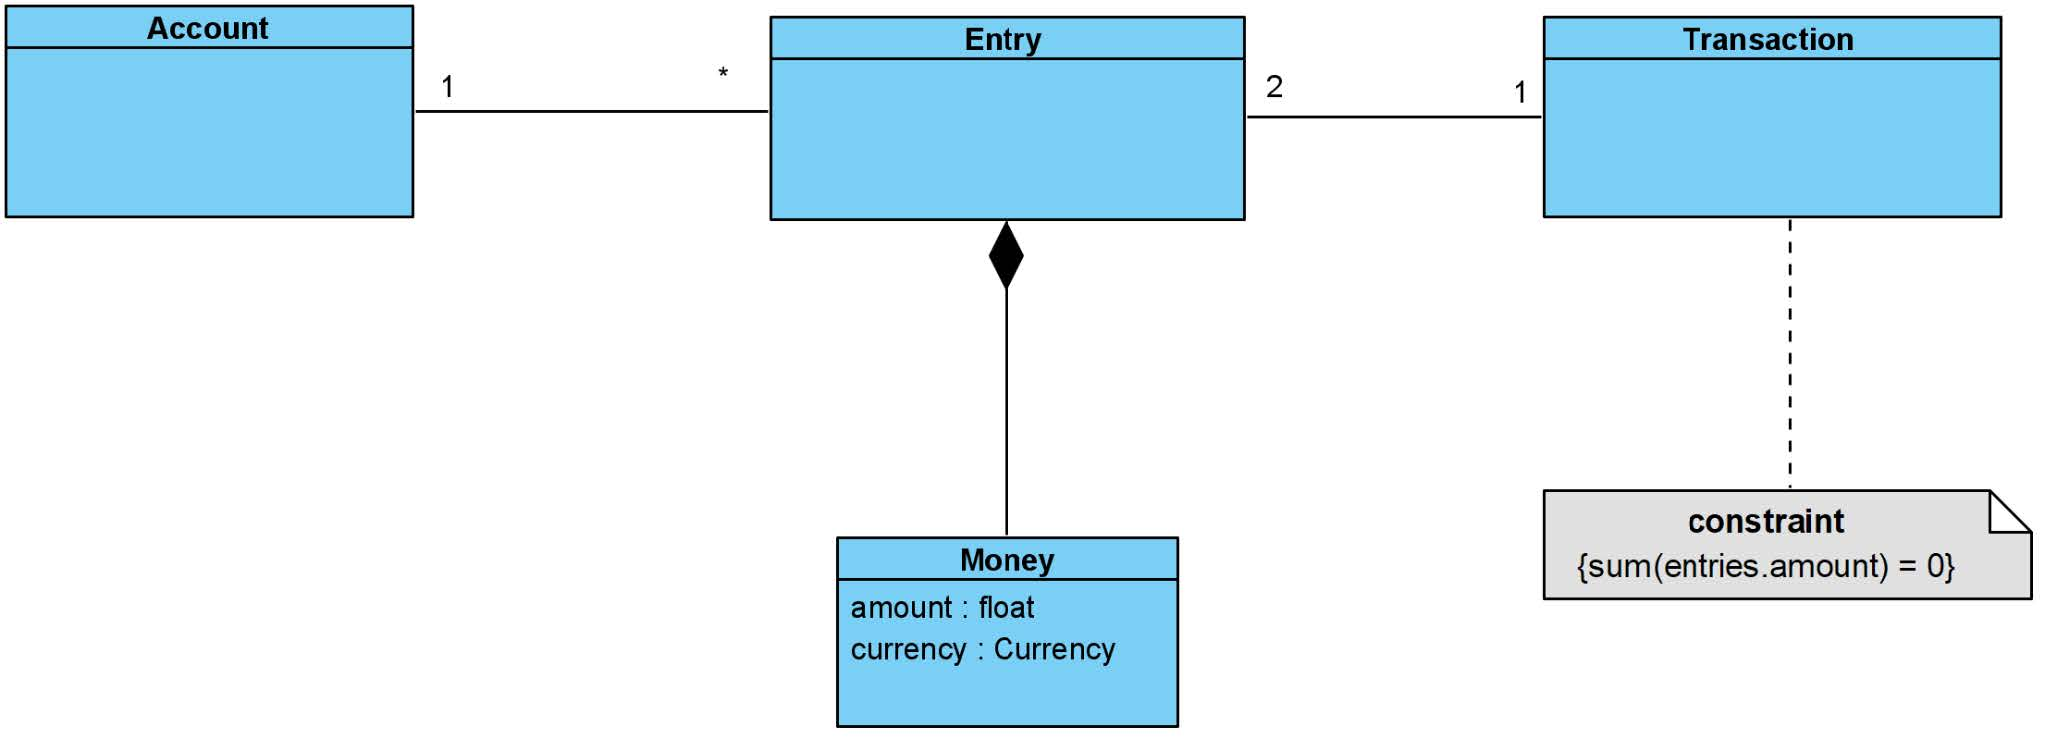
\includegraphics{pic2.jpg}
	\label{fig:label4}
\end{figure}

\subsection*{۳. توجیه بهبود‌ها}
دو مورد از بهبود‌هایی که این الگو به ارمغان می‌آورد را توجیه کنید.

\section*{جواب سوال ۴}

\subsection*{جواب بخش اول}

\begin{figure}[H]
	\centering
	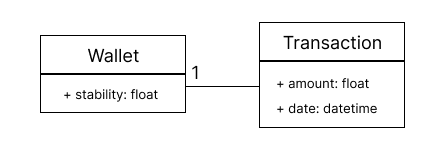
\includegraphics{pic3.png}
	\label{fig:label4}
\end{figure}

\subsection*{جواب بخش دوم}

\begin{figure}[H]
	\centering
	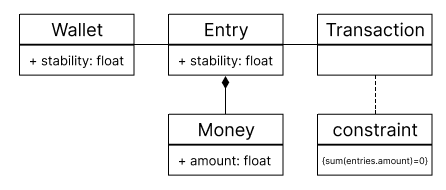
\includegraphics{pic4.png}
	\label{fig:label4}
\end{figure}